\documentclass[12pt,hidelinks]{article}
\author{Rien Maertens\\
    2\textsuperscript{de} Bachelor Informatica}
    \title{Project Zeepbelbomen}
    \usepackage[document]{ragged2e}
    \usepackage[utf8]{inputenc}
    \usepackage[dutch]{babel}
    \usepackage{amsthm}
    %\usepackage[a4paper]{geometry}
    %\geometry{tmargin=2.5cm, bmargin=2.5cm, lmargin=2.5cm, rmargin=2.5cm}
    \usepackage{hyperref}
    \usepackage{enumerate}
    \usepackage{mathtools}
    \usepackage{graphicx}
    \usepackage{float}
    \usepackage{tikz}
    \usepackage{pgfplots}
    \usepackage{pgfplotstable}
    \usepackage{perpage} %the perpage package
    \MakePerPage{footnote} %the perpage package command
    \pgfplotsset{compat=1.10}
    \usetikzlibrary{shapes.geometric,arrows,fit,matrix,positioning}
    \tikzset
    {
        tr/.style = {circle, draw=black, align=center, minimum size=1cm}
    }
    \DeclarePairedDelimiter\floor{\lfloor}{\rfloor} 

    \newtheorem{opgave}{Opgave}
    \newtheorem{geval}{Geval}[subsection]
    \newtheorem{stelling}{Stelling}
    \newtheorem{deelresultaat}{Deelresultaat}
    \hyphenpenalty=10000
    \begin{document}
    \maketitle
    \newpage
    \part{Theoretische Vragen}
    \begin{opgave}
        Geen top in een bladzeepbel heeft een kind in een andere zeepbel.
        \begin{proof}
            Stel we hebben een bladzeepbel $\alpha$ met een top $T$ die een kind $K$ heeft in zeepbel $\beta$. 
            Neem $n$ het aantal zeepbellen dat het pad van zeepbel $\alpha$ naar de wortel bevat. 
            We kunnen de volgende twee gevallen onderscheiden:
            \begin{description}
                \item[Geval 1] Zeepbel $\beta$ bevat een top zonder kinderen en is dus een bladzeepbel.
                    Het pad van de wortel van de boom naar $\beta$ gaat door $\alpha$.
                    Dit pad bevat dus $n+1$ zeepbellen. Dit is tegenstrijdig met het gegeven dat het pad van de wortel naar alle bladzeepbellen evenveel zeepbellen bevat.
                    Het gestelde is dus vals. Het is onmogelijk voor een bladzeepbel om een kind te hebben in een andere zeepbel.
                \item[Geval 2] Zeepbel $\beta$ is geen bladzeepbel, maar bevat wel een pad naar een top zonder kinderen.
                    Deze top is onderdeel van bladzeepbel $\gamma$.
                    Het pad van $\gamma$ naar de wortel van de zeepbelboom bevat $n+k$ zeepbellen, met $k$ het aantal zeepbellen in het pad tussen $\beta$ en $\gamma$.
                    Dit is opnieuw tegenstrijdigi met het gegeven dat het pad van de wortel naar alle bladzeepbellen hetzelfde aantal zeepbellen bevat.
                    Ook in dit geval kan een bladzeepbel geen kinderen in andere zeepbellen hebben.
            \end{description}
        \end{proof}
    \end{opgave}
    \begin{opgave}
        Wat is de maximale diepte van een $k$-zeepbelboom met $n$ sleutels?
        \begin{enumerate}[a.]
            \item Gemeten in zeepbellen. 


                \begingroup 
                \normalfont
                Stel $d_z$ de diepte in zeepbellen van een zeepbelboom. $d_z$ bereikt een maximum wanneer iedere zeepbel maar één top omvat,
                m.a.w. wanneer het pad van de wortel naar een blad evenveel zeepbellen als toppen bevat. 
                De maximale diepte $d_z$ in zeepbellen van een $k$-zeepbelboom met $n$ sleutels is dus gelijk aan de maximale diepte in toppen van een complete binaire boom met $n$ toppen. Dit is dus:
                \begin{equation}
                    d_z \le \floor{\log_2 n}
                \end{equation}
            \endgroup
        \item Gemeten in toppen van de ten gronde liggende binaire boom.


            \begingroup
            \normalfont
            Stel $d_t$ de diepte in toppen van een zeepbelboom. $d_t$ bereikt een maximum wanneer we één lang pad van zeepbellen maken waar elke top van een zeepbel maximum één kind in dezelfde zeepbel bevat. De andere zeepbellen die kinderen zijn van dit lange pad zijn terug zeepbellen met grootte één. Dit ziet er dan als volgt uit:

            \begin{figure}[H]
                \centering


                {
                    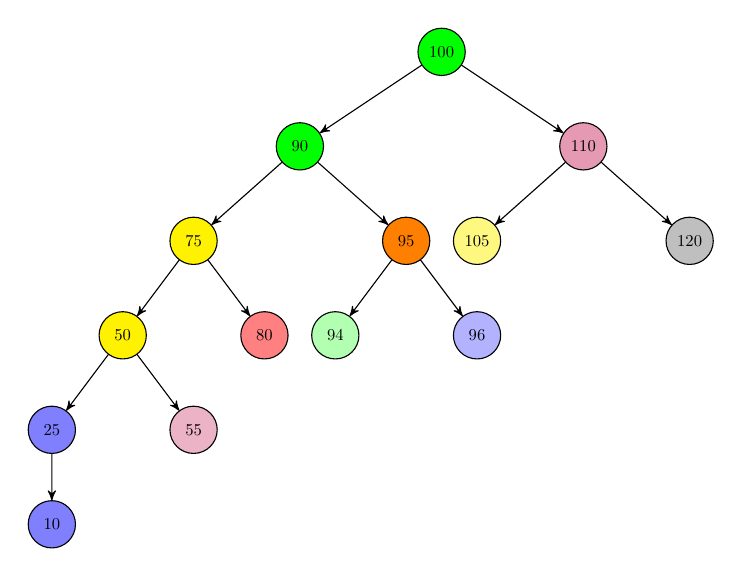
\begin{tikzpicture}[->,>=stealth',
                            level/.style={level distance = 2cm},
                            level 1/.style={sibling distance=6cm},
                            level 2/.style={sibling distance=4.5cm}, 
                            level 3/.style={sibling distance=3cm}, 
                        scale=0.6, transform shape]
                        \node [tr, fill=green] {100}
                        child {
                            node [tr, fill=green] {90} 
                            child {
                                node [tr, fill=yellow] {75} 
                                child {
                                    node [tr, fill=yellow] {50} 
                                    child{
                                        node [tr, fill=blue!50] {25}
                                        child{
                                            node [tr, fill=blue!50] {10}
                                        }
                                    }
                                    child{
                                        node [tr, fill=purple!30] {55}
                                    }
                                }
                                child {
                                    node [tr, fill=red!50] {80} 
                                }
                            }
                            child {
                                node [tr, fill=orange] {95}
                                child{
                                    node [tr, fill=green!30] {94}
                                }
                                child{
                                    node [tr, fill=blue!30] {96}
                                }
                            }
                        }
                        child {
                            node [tr, fill=purple!40] {110}
                            child{
                                node [tr, fill=yellow!50] {105}
                            }
                            child{
                                node [tr, fill=gray!50] {120}
                            }
                        }
                        ;
                    \end{tikzpicture}
                }
            \end{figure}




            Het valt op dat wanneer we een niveau zeepbellen toevoegen, we het dubbele aantal toppen moeten toevoegen van de vorige zeepbelboom met een niveau lager. 
            Voor $n$ het aantal toppen en $z$ het aantal niveaus in zeepbellen geldt: 
            $$n \ge \sum\limits_{i=1}^z k2^{z-1} = k(2^z-1)$$
            We lossen dit op naar $z$: $$z \le \log_2{\left(\dfrac{n+k}{k}\right)}$$
            De maximale diepte $d_t$ van deze zeepbelboom in toppen is gelijk aan het aantal niveaus zeepbellen vermenigvuldigd met het maximale aantal toppen per zeepbel.
            Dus krijgen we dat $d_t=k\cdot z$.
            Wanneer voegen dit alles samen tot één formule:
            \begin{equation}
                d_t \le k \cdot \log_2{\left(\dfrac{n+k}{k}\right)}
                \label{topdiepte}
            \end{equation}
            Waar $d_t$ gelijk is aan de maximale diepte in toppen.
        \endgroup 
\end{enumerate}
    \end{opgave}	
    \begin{opgave}
        Analyse van de verschillende gebalanceerde zeepbelbomen en hun complexiteit.
        \begin{enumerate}[a.]
            \item Voor toevoegen.

                \normalfont
                Het toevoegen van een item aan een gebalanceerde zeepbelboom gebeurt als volgt:

                Eerst wordt het item opgezocht in de zeepbelboom.
                Wanneer het item gevonden werd dan zit het item al in de zeepbelboom en moet er niets gebeuren.
                In dit geval heeft deze bewerking dezelfde tijds- en geheugencomplexiteit als het opzoeken, respectievelijk $O(\log n)$ en $\Theta(1)$ (dit bespreek ik in punt \ref{opzoeken}).

                Als de opzoeking uitkomt op {\tt null} dan zit het toe te voegen item niet in de boom.
                In dit geval wordt er een nieuwe top aangemaakt en bevestigd aan de top die het laatst werd bekeken bij de zoekopdracht.
                De nieuwe top wordt ook toegevoegd aan de zeepbel waarin de ouder zit.
                Indien de zeepbel door deze toevoeging teveel toppen bevat wordt deze gesplitst.
                De manier waarop de zeepbel gesplitst wordt verschilt per implementatie van zeepbelboom:
                \begin{itemize}
                    \item \textbf{Zeepbelboom1} zal zijn zeepbellen splitsen door eerst te kijken of beide kinderen van de wortel in dezelfde zeepbel zitten.
                        Is dit niet het geval dan wordt een rotatie met de bovenste drie zeepbellen uitgevoerd zodat dit wel zo is.
                        Vervolgens wordt de zeepbel gesplitst zodat elk kind van de oude wortel de wortel wordt van een nieuwe zeepbel.
                        De oude wortel wordt daarna toegevoegd aan de zeepbel van zijn ouder, die eventueel opnieuw wordt gesplitst indien deze nu ook overvol zit.
                        Als de oude wortel ook de wortel van de zeebelboom is dan wordt een nieuwe zeepbel aangemaakt.

                        Er wordt enkel binnen dezelfde zeepbel gekeken en omdat de groote van een zeepbel constant is, gebeurt het splitsen van een zeepbel in constante tijd.
                        In het slechtste geval wordt iedere zeepbel vanaf de toegevoegde top tot aan de wortel gesplitst
                        In opgave $2a$ \eqref{topdiepte} hebben we bewezen dat het aantal zeepbellen van de wortel naar een blad maximaal $\floor{\log_2 n}$ is.

                        We kunnen dus concluderen dat voor Zeepbelboom1 met $n$ toppen de toevoegbewerking kost $O(\log n)$ heeft.

                    \item \textbf{Zeepbelboom2} splitst door eerst de zeepbelboom zo goed mogelijk te balanceren. 
                        Hiervoor worden eerst alle toppen in gesorteerde volgorde in een lijst gestoken en vervolgens opgebouwd tot een zo compleet mogelijke binaire boom. 
                        Daarna wordt net zoals Zeepbelboom1 de wortel toegevoegd aan de zeepbel van zijn ouder en vormen de kinderen van deze wortel de wortels van de nieuwe zeepbellen.

                        Net zoals Zeepbelboom1 wordt er enkel binnen dezelfde zeepbel gekeken, echter zal deze zeepbelboom er net iets langer over doen aangezien altijd alle toppen binnen de zeepbel wordt bekeken in plaats van enkel de bovenste drie. 
                        We besluiten dus dat de kost om een een top toe te voegen aan Zeepbelboom2 $O(\log n)$ is voor een boom van $n$ toppen.
                    \item \textbf{Zeepbelboom3} balanceerd net zoals Zeepbelboom2 eerst de toppen in de te grote zeepbel, maar in plaats van enkel de wortel toe te voegen aan de bovenliggende zeepbel worden er meerdere toppen toegevoegd.
                        Hoeveel toppen er toegevoegd worden kan worden aangepast. 
                        Als deze zeepbelboom werd gemaakt met de normale constructor da zullen er zoveel mogelijk toppen worden toegevoegd aan de bovenliggende zeepbel tot deze zijn maximum capactiteit heeft bereikt (maar niet te vol zit).
                        Met een tweede constructor kan er ingesteld worden dat er een maximum staat op het aantal omhoog te duwen toppen en kan dit maximum ook meegegeven worden.
                        Er kan ook ingesteld worden dat er, indien mogelijk, net zoveel toppen aan de bovenliggende zeepbel worden toegevoegd tot deze moet splitsen.

                        Hier geldt hetzelfde als de vorige twee zeepbelbomen: er wordt enkel in dezelfde zeepbel gekeken, wat in constante tijd gebeurt omdat de grootte van de zeepbel constant is.
                        Een splitsing kan een kettingreactie veroorzaken die bovenliggende zeepbellen ook doet splitsen. Maar er zullen maximum $O(\log n)$ van deze splitsingen gebeuren.
                        De toevoegbewerking van Zeepbelboom3 zal dus ook kost $O(\log n)$ hebben voor een boom waar reeds $n$ elementen in zaten
                        opgeslagen.
                \end{itemize}


            \item Voor opzoeken. \label{opzoeken}

                \normalfont
                De drie gebalanceerde zeepbelbomen gebruiken alledrie dezelfde opzoekmethode, dus de complexiteit van deze bewerking is dezelfde.
                Deze methode werkt zoals een normale binaire zoekboom: 

                De wortel wordt vergeleken met het gezochte item. Is het item in de wortel kleiner dan dalen we af naar het rechterkind van de wortel. 
                Is het item in de wortel groter dan dalen we af naar het linkerkind van de wortel.
                Komt de waarde van de wortel overeen met dat van het gezochte item dan hebben we het item gevonden en kunnen we terugkeren uit de functie.
                We blijven op deze manier zoeken tot we het gezochte item gevonden hebben of tot we niet meer verder kunnnen afdalen in de zoekboom (als we null tegenkomen).
                In dit geval zit het gezochte item niet in de zeepbelboom.

                In het slechtste geval zit het item dat wordt gezocht niet in de zeepbelboom en moeten we helemaal tot een blad van de boom afdalen.
                In \eqref{topdiepte} heb ik de maximale diepte in toppen berekend.
                In die formule is $k$ is een constante dus valt die in asymptotische notatie weg.
                We kunnen dus besluiten dat het opzoeken van een element in een gebalanceerde zeepbelboom die $n$ items bevat een kost van $O(\log n)$ heeft.
        \end{enumerate}
    \end{opgave}
    \begin{opgave}
        Bepaal voor semi-splay zeepbelbomen de slechtste-geval complexiteit en de geamortiseerde complexiteit.
        \\ \vspace{0.5em} \normalfont 
        We introduceren eerst een paar stellingen die we zullen gebruiken in de antwoorden van deze opgave:
        \begin{stelling}Het langste pad van de wortel naar een blad in een semi-splay zeepbelboom is naar boven begrens door $O(\log(n))$ \label{stelling1}
            \begin{proof}Het slechtste geval doet zich voor wanneer alle zeepbellen op één lijn staan.
                De lengte van het pad van de wortel naar de top die zich het verst van de wortel bevind is dan gelijk aan het aantal zeepbellen vermenigvuldigd met de maximale diepte van een zeepbel.
                \\
                Het aantal zeepbellen $z$ in een zeepbelboom met $n$ toppen en maximaal $k$ toppen per zeepbel is gelijk aan $\floor{n/k}$.
                Aangezien een complete zeepbel altijd gebalanceerd is heeft deze diepte $\log_2{(k)}$. 
                Het langst mogelijke pad van de wortel naar een blad is $\floor{n/k}\cdot\log_2{(k)} = O(n)$ toppen lang.
                \\
                In asymptotische notatie wordt dit $O(\log(n)$. Dit is precies wat we zochten.
            \end{proof}
        \end{stelling}
        \begin{stelling} Een semi-splay bewerking gebeurt in constante tijd. \label{stelling2}
            \begin{proof}
                Wanneer een splaybewerking wordt uitgevoerd worden alle toppen uit de drie geselecteerde zeepbellen in inorde overlopen en in een lijst gestopt.
                Bij het inorde itereren worden er $3\cdot k$ toppen overlopen, me $k$ de maximale grootte van een zeepbel.
                Vervolgens wordt deze lijst opgedeeld in drie lijsten van lengte $k$ en worden van deze lijsten drie complete gebalanceerde zeepbellen gemaakt.
                Deze drie zeepbellen worden daarna aan elkaar bevestigd en terug in de zeepbelboom geplaatst.
                \\
                Omdat er altijd binnen de gegeven drie zeepbelle wordt gekeken zal een semisplay bewering altijd $\Theta(k)$ operaties op toppen nodig hebben.
                Maar omdat de $k$ in een zeepbelboom constant is kunnen we zeggen dat een splaybewerking in constante tijd of $\Theta(1)$ tijd verloopt.
            \end{proof}
        \end{stelling}
        \begin{description}
            \item[Slechtste geval]
                \hfill
                \begin{itemize}
                    \item \textbf{Voor toevoegen}\\
                        Het slechtste geval doet zich voor wanneer het toe te voegen item moet toegevoegd worden als kind van de top die zich het verst van de wortel bevind. 
                        Wanneer dit geval is moeten alle toppen over dit pad overlopen worden om de plaats van de toe te voegen top te vinden.
                        Nadat de plaats werd gevonden wordt het nieuwe item toegevoegd, wat een bewerking van constante tijd is.
                        Als de zeepbel waaraan de nieuwe top is toegevoegd vol zit moet deze gebalanceerd worden. Dit gebeurt ook in constante tijd.
                        Vervolgens wordt er vanuit deze zeepbel tot aan de wortel gesplayed.
                        \\
                        Uit stelling \ref{stelling1} volgt dat dit langste pad naar boven begrensd wordt door $O(n)$ en uit stelling \ref{stelling2} volgt dat een splaybewerking in constante tijd gebeurt.
                        We kunnen dus besluiten dat een toevoegbewerking op een boom waar reeds $n$ toppen in zitten in het slechtste geval $O(n)$ kost.
                    \item \textbf{Voor opzoeken}\\
                        Een opzoekbewerking is erg gelijkend op een toevoegbewerking. 
                        Het enige verschil is dat bij een zoekbewerking geen top wordt toegevoegd.
                        In het slechtste geval verloopt een opzoekbewerking op een boom van $n$ toppen in $O(n)$ tijd.
                \end{itemize}
            \item[Geamortiseerde complexiteit]
                \hfill
                \begin{stelling}
                    Een reeks van $n > 1$ bewerkingen op een initieel lege semi-splay boom heeft een geamortiseerde complexiteit van $O(n \log n)$, dus is de gemiddelde kost $O(\log n)$ per bewerking.
                    \begin{proof}
                        Ik bewijs dit met behulp van de potentiaalmethode. Voor een lege boom definiëren wij $\Phi(T)=0$.
                        Stel dat $T$ niet leeg is. 
                        Voor een zeepbel $z$ in een semi-splay boom $T$ met een willekeurige $k$-waarde definieren we $A_T(z)$ als het aantal zeepbellen in de deelboom bestaande uit
                        $z$ en al zijn nakomelingen in $T$. Bovendien defineër $L_T(z) = \log(A_T(z))$.
                        De potentiaal van een semi-splay zeepbelboom definiëren wij als:
                        \begin{equation}
                            \Phi(T) = \sum _{z\in T}{L_T(z)}
                        \end{equation}
                        De potentiaal wordt gewijzigd in twee gvallen:
                        \begin{enumerate}[1.]
                            \item Als er een zeepbel wordt toegevoegd (nog zonder de boom te herbalanceren)
                            \item Als tijdens het semi-splayen als gevolg van een toevoeg- of opzoekbewerking er deelbomen vervangen worden
                        \end{enumerate}
                        \begin{deelresultaat}
                            Als een nieuwe zeepbel aan de zeepbelboom $T$ wordt toegevoegd en het resultaat is de boom $T'$ dan geldt $$\Phi(T')-\Phi(T')\le\log(|T'|)$$.
                        \end{deelresultaat}

                        \begin{center}
                            \begin{tabular}{ l | l | p{5cm} }
                                & echte kost & gewijzigde kost \\ \hline
                                top toevoegen & kekeke & $\Phi(U MA)$ \\ \hline
                                top opzoeken & lololo &  $\Phi(U PA)$
                            \end{tabular}
                        \end{center}
                    \end{proof}
                \end{stelling}
        \end{description}
    \end{opgave}
    \newpage
    \part{Implementatie}
    Hieronder volgt er een korte uitleg over de interne structuur en algoritmes die
    ik heb gebruikt voor de implementaties van de zeepbelbomen.
    \section{Binaire boom}
    \subsection{Node}
    Mijn binaire boom bestaat intern uit toppen die hun ouder,  linker en
    rechterkind bijhouden. Om problemen met bidirectionele associaties te vermijden kan de verwijzing
    naar de ouder van een top enkel ingesteld worden wanneer deze top als kind wordt
    aangeduid van een andere top met de methodes {\tt setRightChild()} en {\tt setLeftChild()}. Omdat de wortel van de binaire boom natuurlijk geen
    ouder heeft is er ook een methode die deze verwijzing op {\tt null} zet.
    Een top bevat ook een booleaanse waarde {\tt removed} die functioneert als
    grafsteen. Daarnaast bevat iedere top ook een verwijzing naar de zeepbel waartoe die 
    top behoort. De volgende functies hebben wat extra uitleg nodig:\\
        \begin{description}
            \item[\tt traverseInorder()] traverseer in inorde over de kinderen van deze top. Als argumenten wordt er een {\tt consumer} en een {\tt predicate} meegegeven.
                Zodra een top bij het traverseren van de stack komt wordt deze doorgegeven aan de {\tt consumer}. De {\tt predicate} bepaald hoe ver deze iteratie gaat
                (bijvoorbeeld: enkel in dezelfde zeepbel).
            \item[\tt traverseAndAdd()] maakt gebruik van bovenstaande methode om de kinderen van de top toe te voegen aan de collection {\tt nodes} wanneer ze voldoen aan de
                {\tt predicate}. Wanneer een top voldoet maar één van zijn kinderen niet meer, dan wordt dit kind toegevoegd aan de collection {\tt children}.
        \end{description}
    \subsection{Zeepbel}
    Om de toppen in groepjes in te delen bestaat de klasse {\tt Zeepbel}. Deze houdt
    enkel zijn wortel bij en het aantal toppen dat deze bezit. Een zeepbel heeft ook de
    methodes {\tt topAdded()} en {\tt topsRemoved()} die de zeepbel waarschuwen wanneer
    er toppen bijgekomen of weggevallen zijn. Als de methode {\tt balanceBubble} wordt uitgevoerd
    maakt gebruik deze gebruik van de {\tt TreeBuilder} om zijn toppen intern te balanceren.
    \subsection{Zeepbelboom} 
    In de abstracte klasse Zeepbelboom zit de gemeenschappelijke functionaliteit die
    alle zeepbelboom-implementaties delen. Ik geef wat uitleg over de belangrijkste functies:
    \begin{description}
        \item[\tt find()] vind een item in de zeepbelboom. Meer uitleg kunt u terugviinden in de javadoc-header. Deze methode wordt door alle basisbewerkingen gebruikt.
        \item[\tt add()] voegt een item toe aan de zeepbelboom. Wanneer een item nog niet in de boom zat wordt deze door de abstracte methode {\tt addToParent} toegevoegd aan de boom.
            Die methode is abstract {\tt ShrinkingBubbleTree} en {\tt Zeepbelboom4} anders omgaan met volle zeepbellen.
        \item[\tt contains()] geeft {\tt true} terug wanneer een item in de zeepbelboom zit. Het resultaat is {\tt false} wanneer het gezochte item zich niet in de boom bevind of verwijderd is doormiddel van een grafsteen.
        \item[\tt iterator()] geeft een iterator terug over alle items in de zeepbelboom (die niet verwijderd zijn). Deze maakt gebruik van de {\tt traverseInorder}-methode uit {\tt Node}.
        \item[\tt zeepbelIterator()] iterator over de zeepbellen. Deze methode werkt zoals de {\tt iterator()} methode, maar enkel de wortels van zeepbellen worden bekeken
            en vervolgens worden deze zeepbellen toegevoegd aan de iterator.
    \end{description}
    \subsection{ShrinkingBubbleTree}
    De abstracte superklasse voor de gebalanceerde zeepbelbomen. Deze heeft de abstracte methode {\tt shrinkBubble} die per implementatie verschilt.
    Deze methode wordt opgeropen wanneer er zeepbel te vol zit door een toevoegbewerking en moet gesplitst worden.
    De verschillende implementaties maken gebruik van enkele hulpmethodes die in deze klasse gedefinieerd zijn de uitleg van deze hulpmethodes kunt u in de javadoc-headers vinden.
    Verder zijn ook nog deze functies aanwezig:
    \begin{description}
        \item[\tt addToParent()] voegt een item toe aan een gegeven top en de zeepbel van deze top.
            Wanneer deze zeepbel overvol zit wordt de zeepbel gesplitst m.b.v. {\tt shrinkBubble()}.
        \item[\tt remove()] Helaas heb ik een beetje moeten valsspelen en maak ik gebruik van grafstenen om een top te verwijderen uit de boom.
            Wanneer de boom voor de helft bestaat uit verwijderde toppen wordt de boom opnieuw opnieuw opgebouwd door {\tt rebuildTree}.
            Omdat een top niet echt verwijderd wordt is het mogelijk dat er zeepbellen helemaal gevuld zijn, maar dat hun iterator leeg is.
            \\
            Ik heb geprobeerd een echte implementatie te maken, maar ik kwam vast te zitten bij het debuggen. Deze code kun je nog altijd terugvinden in
            commentaar onderaan in deze klasse.
        \item[\tt removeAll()] In plaats van achter iedere verwijdermethode te controleren of de boom opnieuw opgebouwd moet worden gaat deze bulkoperatie
            eerst de gevraagde elementen verwijderen en pas achteraf kijken of de boom moet opnieuw opgebouwd worden. Dit gebeurt omdat deze opbouwoperatie
            tamelijk duur is.
        \item[\tt rebuildTree()] bouwt de zeepbelboom opnieuw op door eerst alle toppen die niet verwijderd zijn in een lijst te stoppen. Ze worden op een \textit{breadth-first} manier
            in deze lijst getoken zodat wanneer ze opnieuw toegevoegd worden de boom min of meer dezelfde balancering heeft. Moest ze gesorteerd in een lijst zitten dan zou de boom
            zwaar naar rechts overhellen wanneer opniew in die volgorde zouden worden toegevoegd.
    \end{description}
    \subsection{TreeBuilder}
    Hulpklasse die wordt gebruikt om van een gesorteerde lijst van toppen een zo goed mogelijk gebalanceerde binaire boom te maken.
    Volgende functies zijn belangrijk:
    \begin{description}
        \item[\tt listToTree()] methode die een gebalanceerde binaire boom maakt van een gesorteerde lijst van toppen. Dit gebeurt op een recursieve manier in $\Theta(n)$ tijd (met $n$ de lengte van de lijst.
        \item[\tt listToTreeIterative()] iteratieve versie van bovenstaande methode. Deze maakt gebruik van een {\tt while}-loop en een stack in plaats van een recursieve oproep.
            Uit testen bleek dat deze methode trager was dan de recursieve methode dus wordt deze functie niet gebruikt.
        \item[\tt attachChildren()] voegt een lijst van $n+1$ toppen toe als kinderen van de bladeren van de opgebouwde boom.
    \end{description}

    \section{Implementaties gebalanceerde zeepbelbomen} 
    Nu volgt een beschrijving van {\tt splitBubble}-methode van de zeepbelbomen die {\tt ShrinkingBubbleTree} implementeren.
    \subsection{Zeepbelboom1}
    Wanneer de wortel van de zeepbel twee kinderen heeft die in dezelfde zeepbel zitten wordt er niets veranderd aan de interne structuur.
    Is dit niet het geval dan wordt er een rotatie uitgevoerd op de bovenste drie toppen tot dit wel zo is.
    Vervolgens worden de twee kinderen van de wortel genomen als nieuwe wortels voor twee nieuwe zeepbellen.
    De oude wortel wordt daarna toegevoegd aan de bovenliggende zeepbel. 
    Als deze top de wortel van de zeepbelboom was, en dus geen bovenliggende zeepbel had, dan wordt er een nieuwe zeepbel aangemaakt en ingesteld als wortelzeepbel.
    Wanneer deze top wel aan een bestaande zeepbel kon toegevoegd worden wordt deze indien nodig opnieuw gesplitst.
    \subsection{Zeepbelboom2}
    Voor de zeepbel gesplitst wordt wordt deze eerst gebalanceerd met {\tt balanceBubble}. Daarna wordt op dezelfde manier gesplitst als
    {\tt Zeepbelboom1}.
    \subsection{Zeepbelboom3}
    Deze zeepbel werkt op dezelfde manier als {\tt Zeepbelboom2} echter worden er hier
    zoveel mogelijk toppen aan de bovenliggende zeepbel toegevoegd. Deze zeepbelboom
    kan geconfigureerd worden: er kan gekozen worden om een maximum te zetten op het 
    aantal omhoog te duwen toppen en er kan ingesteld worden dat er geprobeerd wordt
    om net genoeg toppen toe te voegen aan de bovenliggende zeepbel dat die verplicht
    wordt om te splitsen.  
    \section{Semi-splay zeepbelboom}
    \subsection{Zeepbelboom4}
    Deze zeepbelboom is een implementatie van de semi-splay zeepbelboom. 
    Bij elke toevoeg- en opzoekbewerking wordt er gesplayed op zeepbelniveau vanaf de zeepbel van de top die het werd toegevoegd op opgezocht tot aan de wortelzeepbel.
    Ik geef wat meer uitleg bij de volgende methodes:
    \begin{description}
        \item[\tt addToParent()] voegt een nieuwe top toe aan een top die reeds in de boom zit.
            De nieuwe top wordt toegevoegd aan de zeepbel van de ouder als hier nog plaats in is. 
            Als deze zeepbel door deze toevoeging volledig gevuld is wordt ze gebalanceerd. 
            Is de zeepbel van de ouder al volledig gevuld dan wordt een nieuwe zeepbel aangemaakt met de nieuwe top als wortel.
        \item[\tt find()] doet hetzelfde als de gelijknamige methode van de superklasse, met dat verschil dat na iedere opzoeking en toevoeging er gesplayt wordt.
        \item[\tt semiSplay()] splayt de zeepbellen vanaf de zeepbel van de meegegeven top.
            Dit splayen gebeurt als volgt:
            \begin{enumerate}
                \item Eerst worden de drie zeepbellen geselecteerd die moeten worden gesplayed. Eerst wordt de zeepbel geselecteerd waartoe de meegeven top behoort.
                    Is deze zeepbel niet compleet dan wordt zijn ouderzeepbel in de plaats genomen.
                    Vervolgens worden ook de ouderzeepbel van de laatst geselecteerde zeepbel en zijn ouderzeepbel geselecteerd.
                \item Vervolgens worden de toppen van deze zeepbellen in een lijst gestoken door ze in inorde te overlopen.
                    Ook worden de kindertoppen van deze geselecteerde toppen bijgehouden zodat ze later terug kunnen toegevoegd worden.
                \item Deze lijst wordt vervolgens in drie gedeeld en van deze deellijsten worden er nieuwe zeepbellen gemaakt met de {\tt TreeBuilder}.
                \item Daarna worden deze drie bomen en de kindertoppen uit stap 1 aan elkaar bevestigd.
                \item Als laatste stap wordt de bovenste van deze nieuwe drie zeepbellen geslecteerd om te splayen zodat de volgende iteratie kan beginnen.
            \end{enumerate}
            Deze bewerking herhaalt zich tot de wortelzeepbel of een kindzeepbel van de wortelzeepbel wordt bereikt.
            
    \end{description}
    \newpage
    \part{Experimenten}
    Nu volgen de resultaten van enkele testen die ik heb uitgevoerd op de zeepbelbomen.
    \section*{Opzet}
    Mijn testresultaten heb ik verkregen door gebruik te maken van de volgende klassen:
    \begin{description}
        \item[\tt TestResult]: klasse die de tijden en parameters van de verschillende testen voor een zeepbelboom bijhoud.
            In deze klasse zijn ook een aantal comparators gedefiniëerd zodat kan gesorteerd worden op naam, tijd om iets toe te voegen \ldots
        \item[\tt PerformanceTest]: hier gebeuren de echte testen. 
            Deze klasse heeft twee methodes die verschillende benchmarks uitvoeren:
            \begin{itemize}
                \item {\tt testPerK} gaat alle zeepbelboomimplementaties testen met een verschilende $k$-waarde en een inputgrootte die gelijk blijft.
                \item {\tt testPerN} test de zeepbelbomen met een vaste $k$-waarde, maar met een stijgende inputgrootte.
            \end{itemize}
            Algemeen lopen deze testen als volgt: Eerst wordt de input aangemaakt door een array van integers te maken en door elkaar te shuffelen.
            Vervolgens wordt iedere bewerking---toevoegen, opzoeken en verwijderen indien geïmplementeerd--- tien keer na elkaar uitgevoerd op deze lijst van getallen.
            Om de resultaten zo stabiel mogelijk te houden wordt iedere reeks voorafgegaan door eenzelfde bewerking die niet wordt gemeten.
            Ook wordt iedere keer er een nieuwe boom wordt gebruikt de garbagecollection manueel opgeropen.
        \item[\tt PerformanceWriter]: deze klasse bevat de {\tt main()} methode voor de experimenten. Zowel {\tt testPerK} als {\tt testPerN} worden uitgevoerd en de resultaten hiervan worden uitgeschreven naar bestanden.
    \end{description}
    Om de meetresultaten zo stabiel mogelijk te houden heb ik het gehele project gecompileerd in een {\tt jar}-bestand.
    Dit gecompileerde bestand heb ik vervolgens een paar uur laten draaien op een linux-machine.
    Doormiddel van de kernel-parameter {\tt isolcpus} heb ik één processorkern gereserveerd zodat ik met {\tt taskset} de experimenten heb kunnen uitvoeren op enkel deze processorkern zonder dat andere processen konden interferen.

    \section*{Resultaten}
    De resultaten van de meetresultaten door de voorgaande tests kun je in de volgende grafiekjes zien:
    \subsection*{Gebalanceerde zeepbelbomen}
    \begin{figure}[H]
        \begin{tikzpicture}
            \begin{axis}[title=Add, xlabel=$k$-waarde, ylabel=Tijd (ms), ymax=800, legend pos=north east, scaled ticks=false, width=13cm, height=7cm, /pgf/number format/.cd, use comma]
                \addplot +[mark=*] table [x=k, y=add]{testresults/Zeepbelboom1_K500_Ktest.dat};
                \addlegendentry{Zeepbelboom1}
                \addplot +[mark=*] table [x=k, y=add]{testresults/Zeepbelboom2_K500_Ktest.dat};
                \addlegendentry{Zeepbelboom2}
                \addplot +[mark=*] table [x=k, y=add]{testresults/Zeepbelboom3_K500_Ktest.dat};
                \addlegendentry{Zeepbelboom3}
            \end{axis}
        \end{tikzpicture}\caption{Toevoegen van $100.000$ items aan een gebalanceerde zeepbelboom. }
        \label{figAdd}
    \end{figure}

    \begin{figure}[H]
        \begin{tikzpicture}
            \begin{axis}[title=Contains, xlabel=$k$-waarde, ylabel=Tijd (ms), ymax=600, legend pos=north east, scaled ticks=false, width=13cm, height=7cm, /pgf/number format/.cd, use comma]
                \addplot +[mark=*] table [x=k, y=contains]{testresults/Zeepbelboom1_K500_Ktest.dat};
                \addlegendentry{Zeepbelboom1}
                \addplot +[mark=*] table [x=k, y=contains]{testresults/Zeepbelboom2_K500_Ktest.dat};
                \addlegendentry{Zeepbelboom2}
                \addplot +[mark=*] table [x=k, y=contains]{testresults/Zeepbelboom3_K500_Ktest.dat};
                \addlegendentry{Zeepbelboom3}
            \end{axis}
        \end{tikzpicture}
        \caption{Opzoekactie in een gebalanceerde zeepbelboom met $100.000$ items.}
        \label{figCont}
    \end{figure}
    \begin{figure}[H]
        \begin{tikzpicture}
            \begin{axis}[title=Remove, xlabel=$k$-waarde, ylabel=Tijd (ms), ymax=600, legend pos=north east, scaled ticks=false, width=13cm, height=7cm, /pgf/number format/.cd, use comma]
                \addplot +[mark=*] table [x=k, y=remove]{testresults/Zeepbelboom1_K500_Ktest.dat};
                \addlegendentry{Zeepbelboom1}
                \addplot +[mark=*] table [x=k, y=remove]{testresults/Zeepbelboom2_K500_Ktest.dat};
                \addlegendentry{Zeepbelboom2}
                \addplot +[mark=*] table [x=k, y=remove]{testresults/Zeepbelboom3_K500_Ktest.dat};
                \addlegendentry{Zeepbelboom3}
            \end{axis}
        \end{tikzpicture}\caption{$100.000$ elementen verwijderen uit een gebalanceerde zeepbelboom.}
        \label{figRem}
    \end{figure}
    \paragraph{Toevoegen}
    Voor de toevoegbewerking merken we in figuur \ref{figAdd} dat de Zeepbelboom1 de beste tijden heeft.
    Dit komt doordat er veel minder toppen van plaats worden veranderd in de ondeliggende boom.
    De tweede en derde implementatie duren meestal langer omdat bij iedere splitsing de gehele zeepbel wordt gebalanceerd.
    Zeepbelboom3 presteert dan weer beter dan de tweede omdat door meerdere toppen toe te voegen aan de ouderzeepbel, er meer plaats is in de nieuwe zeepbellen.
    Hierdoor zullen er minder splitsingsacties moeten gebeuren en is de toevoegbewerking dus sneller.
    \paragraph{Opzoeken}
    Op figuur \ref{figCont} zien we dat Zeepbelboom1 nu de slechtste tijden heeft.
    Omdat er hier zo weinig mogelijk wijzigingen gedaan worden is deze boom intern minder gebalanceerd dan de andere twee implementaties.
    Het kan dus langer duren om in Zeepbelboom1 een opzoeking te doen dan bij Zeepbelboom2 en Zeepbelboom3.
    Zeepbelboom2 presteert beter dan zeepbelboom3 want deze zeepbelboom zal minder zeepbellen bevatten, waardoor de boom in het algemeen ook gebalanceerder is.
    \paragraph{Verwijderen}
    De verwijderactie in mijn gebalanceerde zeepbelbomen komt eigenlijk neer op een simpele opzoekactie gevolgd door eventueel een booleanse waarde die moet veranderd worden.
    Daarom kunnen we op figuur \ref{figRem} zien dat de tijden van de verwijderbewerking overeen komen met die van de opzoeking.
    

    \subsection*{Zeepbelboom3}
    \begin{figure}[H]\begin{tikzpicture}
            \begin{axis}[title=Zeepbelboom3, xlabel=$k$-waarde, ylabel=Tijd (ms), ymax=700,  legend pos=north east, scaled ticks=false, width=13cm, height=7cm, /pgf/number format/.cd, use comma]
                \addplot +[mark=*] table [x=k, y=add]{testresults/Zeepbelboom3_K500_parentOverflow_Ktest.dat};
                \addlegendentry{Parent overflow}
                \addplot +[mark=*] table [x=k, y=add]{testresults/Zeepbelboom3_K500_maxPushUp5_Ktest.dat};
                \addlegendentry{Max.5}
                \addplot +[mark=*] table [x=k, y=add]{testresults/Zeepbelboom3_K500_maxPushUp5_parentOverflow_Ktest.dat};
                \addlegendentry{Max. 5 en p.o.}
                \addplot +[mark=*] table [x=k, y=add]{testresults/Zeepbelboom3_K500_Ktest.dat};
                \addlegendentry{Normaal}
            \end{axis}
        \end{tikzpicture}
        \caption{De verschillende configuraties van Zeepbelboom3.}
        \label{figZB3}
    \end{figure}
    op figuur \ref{figZB3} kunnen we zien dat het verschil tussen een boom met parent overflow\footnote{Indien mogelijk worden er zodanig veel toppen toegevoegd aan de ouderzeepbel dat deze verplicht is zich ook te splitsen.} (afgekort p.o.) aan en uit niet significant is. We kunnen wel een verschil zien tussen de zeepbelboom waar een maximum staat op het aantal toppen
    die toegevoegd mag worden aan de ouderzeepbel.
    Bij een lage $k$-waarde presteerd deze iets slechter omdat er door één splitsingsactie terug minder nieuwe zeepbellen bijkomen waardoor er vlugger gesplitst zal moeten worden.
    Wanneer deze $k$ groter wordt is dit maximum beter. Er is namelijk een punt waarop er teveel nieuwe zeepbellen worden aangemaakt en deze splitsingsactie trager zal verlopen.
    \section*{Semi-splay zeepbelbomen}
    \begin{figure}[H]
        \begin{tikzpicture}
            \begin{axis}[title=Semi-splay zeepbelboom, xlabel=$k$-waarde, ylabel=Tijd (ms), legend pos=north east, scaled ticks=false, width=13cm, height=7cm, /pgf/number format/.cd, use comma]
                \addplot +[mark=*] table [x=k, y=add]{testresults/Zeepbelboom4_K500_Ktest.dat};
                \addlegendentry{add}
                \addplot +[mark=*] table [x=k, y=contains]{testresults/Zeepbelboom4_K500_Ktest.dat};
                \addlegendentry{contains}
            \end{axis}
        \end{tikzpicture}
        \caption{Semi-splay zeepbelboom}
        \label{figSemi}
    \end{figure}
    Ik was enorm verbaasd toen ik figuur \ref{figSemi} zag. 
    Zoals verwacht is een grotere $k$-waarde trager voor het toevoegen en opzoeken, er moeten telkens meer bewerkingen op toppen uitgevoerd worden per splaybewerking.
    Waardoor iedere splaybewerking meer tijd zal innemen hoe groter de $k$-waarde is.
    \\
    Maar bij een $k$ van 150 (en eigenlijk al vanaf 100) doet er zich iets vreemd voor: de toevoeg- en opzoekbewerking verloopt enorm veel vlugger en stijgt ook minder snel in functie van $k$.
    Bij het bespreken van deze merkwaardige resultaten met medeleerlingen hebben ze mij verteld dat hun Zeepbelboom4 ongeveer hetzelfde gedrag vertoond, alleen is het bij mij wel erg extreem.
    Ik heb helaas geen tijd meer om dit fenomeen te onderzoeken, maar waarschijnlijk zit er ergens een fout in mijn code.
    \section*{Besluit}
    Zeepbelbomen zijn een manier om binaire bomen min of meer gebalanceerd te houden. Zeepbelboom1 presteerd het beste wanneer er veel toevoegingen gebeuren.
    Als er meer opzoekingen gebeuren is het beter om Zeepbelboom2 te gebruiken.
    Zeepbelboom3 is een middenweg, maar ik kan aanbevelen om een maximum mee te geven wanneer een grote $k$-waarde wordt gebruikt.
    Ten slotte kan ik u afraden om de semi-splay zeepbelboom te gebruiken. Het is namelijk enorm traag, zelfs voor een kleine $k$. Daarnaast vertrouw ik mijn eigen implementatie ook niet genoeg.
    \end{document}
